%_____________________________________________________________________________
%
%STRUTTURA RELAZIONE:
%
%istituto
%scopo -DONE
%introduzione teorica
%strumentazione  -DONE
%procedimento     
%dati sperimentali con tab
%elaborazione dati = calcoli teorici
%conclusione = confronto risultati teorici con dati sperimentali
%
%_____________________________________________________________________________

%NOTA UTILE: se in un testo bisogna inserire qualche dato numerico in riga, senza
%dover ricorrere a \begin{equation}, basta includere cio' che serve dentro a $....$
%esempio: $10k\Omega$ per inserire il dato in Ohm, poichè alcuni caratteri non vengono presi se stanno fuori da un'equazione


\documentclass{article}
\usepackage{amsmath}
\usepackage{setspace}
\usepackage{anysize}
\usepackage{geometry}
\usepackage{epsfig}
\usepackage{graphicx}
%c'è 1 inch di margine a destra e sinistra
%\geometry{margin = 1.25 in}

\title{\huge Relazione prima esperienza di laboratorio Fisica 2}
\author{Gruppo A15: Armani Stefano, Cappellaro Nicola, Pasquato Leonardo}
\date{10-10-2022}
\setlength{\parindent}{0cm}

\begin{document}
    %print sezione titolo
    \maketitle
    \rule{\linewidth}{0.1mm}

    %scopo  Stefano
    \section{Scopo dell'esperienza}
    Lo scopo della prima esperienza di laboratorio è stato quello di verificare sperimentalmente ciò che è stato
    illustrato solamente in teoria, in modo tale da valutare le discrepanze tra i risultati sperimentali e i risultati attesi dai calcoli ideali.
    I circuiti costruti sono stati utilizzati per verificare sperimentalmente le leggi base dell'elettrotecnica, ossia la legge di Ohm,
    le leggi di Kirkhhoff, la legge di Millman. \par
    Lo scopo implicito di questa esperienza è stato quello di familiarizzare con gli strumenti del laboratorio come il generatore da banco,
    breadboard, multimetro e componenti elettronici. 
    
        
    %introduzione teorica   Nicola
    \section{Cenni teorici}
    In questa prima esperienza di laboratorio sono studiate e verificate la legge di Ohm utilizzando i resistori e le leggi di Kirchhoff: in particolare nel secondo esperimento
    sarà verificato il teorema di Millman per le reti elettriche. \par
    Ricordiamo:
    \begin{itemize}
        \item Legge di Ohm $V = R \cdot I$, ossia la legge caratteristica dei \textit{resistori};
        \item Legge di Kirchhoff delle correnti $\sum_{e = 1}^{n} i_e = \sum_{u = 1}^{m} i_u $;
        \item Legge di Kirchhoff delle tensioni $\sum_{k = 1}^{n} V_k = 0 $;
        \item Teorema di Millman $V_0 = \frac{\sum_{k = 1}^{n} \frac{V_k}{R_k} }{\sum_{k = 1}^{n} \frac{1}{R_k} }$, ossia una diretta conseguenza delle leggi di Kirchhoff: la tensione ai terminali di un circuito comuni ad \textit{n} rami
                corrisponde al rapporto tra la somma algebrica delle correnti cortocircuitate dei rami presi singolarmente e la somma dei reciproci delle resistenze.
    \end{itemize}
    I circuiti realizzati sono di tipo lineare a tempo invariante e sono detti LTI, quindi i loro comportamenti sono idealmente costanti nel tempo.
    
    
    \newpage
    %elenco strumentazione                          INSERISCI PORTATA E SENSIBILITÀ
    \section{Strumentazione}
    \begin{itemize}
        \item Breadboard con annessi morsetti serrafilo;
        \item Cavi con connettori a banana;
        \item Resistori di varie misure ($1k\Omega$, $10k\Omega$, $100k\Omega$, $1M\Omega$, $10M\Omega$);
        \item Connettori da banco (Jumper);
        \item Multimetro;
        \item Alimentatore da banco (generatore di corrente e tensione).
    \end{itemize}

    %descrizione esperimento    Leonardo
    \section{Esperimento}
    Una volta messo a disposizione il kit contenente la strumentazione indicata al punto $3$, %fai link
    si è esposto il primo esercizio riguardante un semplice \textbf{partitore di tensione}.
    Il partitore di tensione è un circuito LTI di prim'ordine come in figura, composto da
    generatore di tensione, 2 resistori in serie ed un multimetro collegato in parallelo al secondo resistore.

    %\FloatBarrier foto schematico
    \begin{figure}[!h]            %[!h] = inserimento forzato dell'immagine sotto il titoletto della section
        \begin{center}
            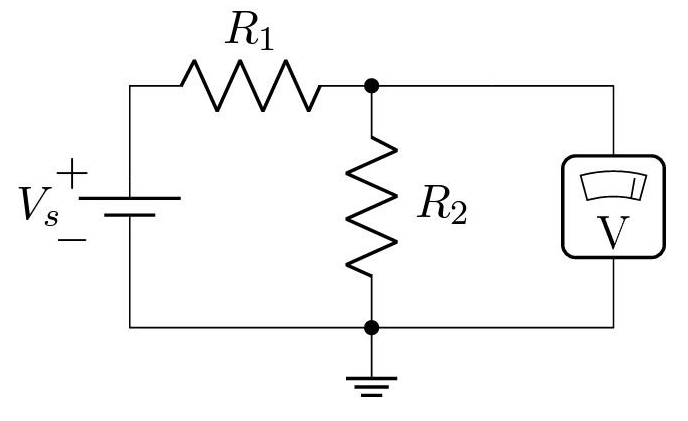
\includegraphics[width = 5cm]{ese1.png}
            \caption{Partitore di tensione}
            \label{ese1}
        \end{center}
    \end{figure}
    

    %INSERISCI FIGURA DELLO SCHEMATICO DEL CIRCUITO + FOTO REALE
    Si è successivamente replicato lo stesso circuito su una \textbf{Breadboard} utilizzando due resistori da
    $1k\Omega$, connettori da banco per collegare la Breadboard ai morsetti serrafilo connessi al generatore
    tramite \textbf{connettori a banana}. \par
    Successivamente sono stati accesi il multimetro e il generatore e per prima cosa sono stati impostati i limiti di corrente e tensione massima
    erogabile dal generatore, rispettivamente a $6mA$ e $6V$.\par
    A questo punto è stato possibile attivare il generatore affinchè nel circuito venisse mantenuta la tensione voluta e,
    grazie al multimetro impostato in modo tale da fungere da voltmetro, è stato possibile ottenere la tensione di lato della
    seconda resistenza in serie. La tensione di lato ottenuta è stata pari a $3.020V$.
    Successivamente, è stato ripetuto lo stesso esperimento utilizzando diversi resistori, ottenendo risultati leggermente diversi.\par
    I risultati più discostati dai precedenti sono sicuramente stati rilevati nelle ultime due misurazioni in cui sono stati utilizzati
    resistori con resistenze ben più alte rispetto alle precedenti (nell'ordine dei $M\Omega$).\par
    \par
    \newpage
    Nella seconda parte di questa esperienza di laboratorio è stato illustrato dal punto di vista teorico
    un teorema derivante dalle leggi di \textbf{Kirchhoff}, ossia il teorema di \textbf{Jacob Millman}.
    Dopo un'illustrazione teorica, è stato esposto un secondo esercizio in cui si può verificare sperimentalmente il teorema di Millman:
    
    %foto esercizio e foto circuito
    \begin{figure}[!h]
        \begin{center}
            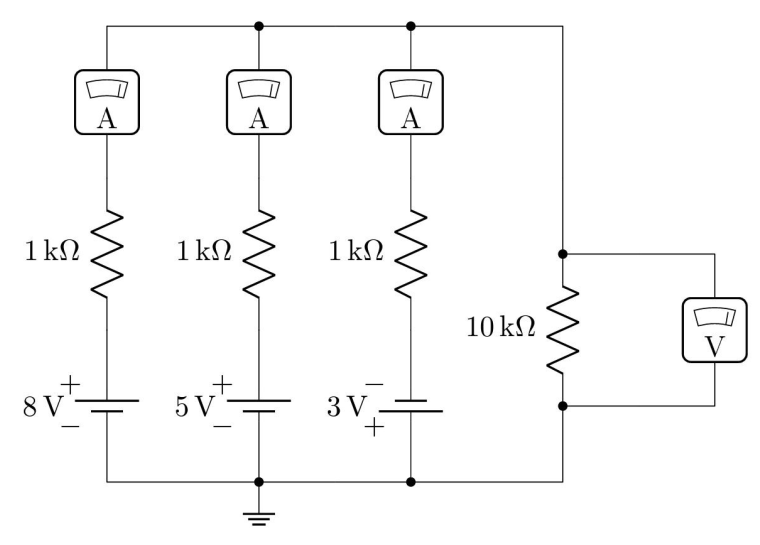
\includegraphics[width = 6cm]{ese2.png}
            \caption{Secondo circuito}
            \label{ese2}
        \end{center}
    \end{figure}

    Una volta costruito il circuito sono state ripetute 3 misurazioni da parte del multimetro impostato come 
    amperometro, in modo tale da poter misurare sperimentalmente le correnti uscenti dai resistori collegati ai rispettivi generatori.\par
    Ottenuti i valori delle correnti, è stata valutata la tensione di lato ($V_M$) sulla resistenza da $10k\Omega$, come in figura:
    Questa misurazione sperimentale è prossima alla tensione teorica calcolata tramite il teorema di Millman.\par



    %risulati sperimentali          INSERISCI ERRORI, CHIEDI PROF
    \section{Dati sperimentali}
    \begin{center}
        Primo esperimento: \par
    \begin{tabular}{|c|c|c|c|}
        \hline
        \textit{Test} & \textit{Primo resistore} & \textit{Secondo resistore} & \textit{Tensione di lato} \\
        \hline
        Test 1 & $R_1 =1k\Omega$ & $R_2=1k\Omega$ & $V_1=3,020.65V$\\
        \hline
        Test 2 & $R_1 =1k\Omega$ & $R_2=500\Omega$ & $V_2=2,011.25V$\\
        \hline
        Test 3 & $R_1 =10k\Omega$ & $R_2=10k\Omega$ & $V_3=3,007.85V$\\
        \hline
        Test 4 & $R_1 =100k\Omega$ & $R_2=100k\Omega$ & $V_4=2,987.50V$\\
        \hline
        Test 5 & $R_1 =1M\Omega$ & $R_2=1\Omega$ & $V_5=2,857.62V$\\
        \hline
        Test 6 & $R_1 =10\Omega$ & $R_2=10\Omega$ & $V_6=1,836.33V$\\
        \hline
    
    \end{tabular}
    \end{center}
    
    \begin{center}
        Secondo esperimento: \par
    \begin{tabular}{|c|c|c|}
        \hline
        \textit{Ramo cortocircuitato} & \textit{Tensione} & \textit{Intensità di corrente} \\
        \hline
        Primo ramo & $V_1 = 8V$ & $I_1 = 4,782.75 mA$\\
        \hline
        Secondo ramo & $V_2 = 5V$ & $I_2 = 1,695.85 mA$\\
        \hline
        Terzo ramo & $V_3 = -3V$ & $I_3 = 6,276.95 mA$\\
        \hline
        & $V_M = 3,198.98V$&\\
        \hline
    
    \end{tabular}
    \end{center}


    \newpage

    %elaborazione dati  Leonardo
    \section{Elaborazione dati}
    Primo esperimento, $V_s = 6V$:
    \begin{align}
        I_s = \frac{V_s}{R_{eq}}  \hspace{2cm}   & v_{R_2} = \frac{V_s}{V_{eq}} \cdot R_2  \hspace{2cm} &  V_{eq} = R_1 + R_2 \\
        & V_{Test1} = \frac{6V}{1k\Omega + 1k\Omega} \cdot 1k\Omega = 3V \\
        & V_{Test2} = \frac{6V}{1k\Omega + 500\Omega} \cdot 500\Omega = 2V \\
        & V_{Test3} = \frac{6V}{10k\Omega + 10k\Omega} \cdot 10k\Omega = 3V \\
        & V_{Test4} = \frac{6V}{100k\Omega + 100k\Omega} \cdot 100k\Omega = 3V \\
        & V_{Test5} = \frac{6V}{1M\Omega + 1M\Omega} \cdot 1M\Omega = 3V \\
        & V_{Test6} = \frac{6V}{10M\Omega + 10M\Omega} \cdot 10M\Omega = 3V
    \end{align}

    Secondo esperimento:
    \begin{align}
       & V_M = \frac{\frac{V_1}{R_1} + \frac{V_2}{R_2} + \frac{V_3}{R_3}}{\frac{1}{R_1} + \frac{1}{R_2} + \frac{1}{R_3} + \frac{1}{R_4}}\\
       & V_M = \frac{\frac{8V}{1k\Omega} + \frac{5V}{1k\Omega} + \frac{-3V}{1k\Omega}}{\frac{1}{1k\Omega} + \frac{1}{1k\Omega} + \frac{1}{1k\Omega} + \frac{1}{10k\Omega}} = 3,226V
    \end{align}
    


    %conclusione
    \section{Conclusione}
    Nel primo esperimento sono stati ottenuti dei valori di tensione prossimi a quelli ideali con i resistori inferiori ad $1M\Omega$.
    Nel momento in cui sono stati utilizzati resistori con resistenze dell'ordine dei $M\Omega$, sono emersi valori distanti dal risultato teorico.
    Questo succede a causa della resistenza interna del voltmetro $R_{intV}$: posizionato il voltmetro in parallelo alla seconda resistenza, sono state rilevate grosse variazioni
    perchè le resistenze $R_1$ e $R_2$ avevano valori prossimi all'incognita resistenza interna del voltmetro, dunque quest'ultima ha agito come una vera e propria
    resistenza in parallelo a $R_2$. Questa anomalia non è stata rilevata con i resistori precedenti poichè avevano resistenze di ordini ben minori rispetto alla resistenza
    interna del voltmetro, dunque la maggior intensità della corrente percorreva i resistori $R_1$ e $R_2$ (Vedi legge di Ohm).\par
    È stato quindi possibile calcolare in modo approssimativo $R_{intV}$, considerando $V_{in} = V_6 \approx 2V$ :
    \begin{equation}
        \frac{V_{out}}{V_{in}} = \frac{R_{eqV}}{R_1 + R_{eqV}} = \frac{6V}{2V} = \frac{1}{3} \longrightarrow R_{eqV} = \frac{R_1}{2} = \frac{10M\Omega}{2} = 5M\Omega
    \end{equation}
    dove $R_{eqV}$ è il parallelo tra $R_2$ e $R_{intV}$.\par
    La resistenza interna del multimetro $R_{intV}$ dunque risulta essere pari a $10M\Omega$

    Nel secondo esperimento è stato verificato il teorema di Millman: dopo aver misurato sperimentalmente il valore della tensione di lato ai morsetti comuni,
    è stata confrontata questa misurazione con il valore atteso. La valutazione è stata positiva: il valore sperimentale era prossimo al valore ideale.

\end{document}